\setchapterpreamble[o]{%
  \dictum[Steve Jobs]{\textit{``Design is not  just what it looks like and
      feels like. Design is how it works.''}}}

\chapter{Design and Implementation}
\label{cha:design}


\section{Architecture}
\label{sec:architecture}

This  section  introduces  the  desired architecture  of  the  ``Xen-based
execution     environment''.      The     system    as     depicted     in
Figure~\ref{fig:architecture}   essentially   consists   of  the   following
components:
\begin{enumerate}
  
\item some kind of a user --- that could be a real person using the system
  on  one hand  or  a script  or some  other  program such  as a  ``Calana
  Broker''        (described        in        \cite{dalheimer05agentbased,
    dalheimer06calanaprotocol}) on the other hand.
  
\item a central  managing daemon running on a Xen  \cite{xen} host or more
  concretely within \texttt{dom0}.  This part is, for instance, accessible
  through a command line, a web service or some other interface. A user in
  general  does  only   talk  directly  to  this  part   of  the  system.  
  Figure~\ref{fig:architecture} shows this part  as the ``Xen Manager''.
  
\item the third component resides  directly on a Xen instance and provides
  several functions to the  managing daemon (``Xen instance controller''). 
  Functionalities  of this component  include: monitoring  and controlling
  the user's  application, mounting external data  locations and providing
  access to generated results.

\end{enumerate}

\begin{figure}[htbp]
  \begin{center}
%    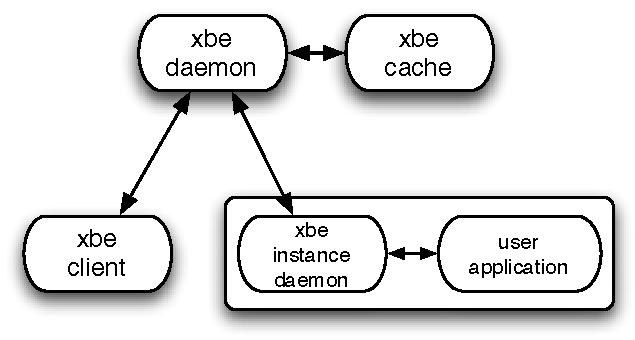
\includegraphics[height=80mm]{architecture-overview}
  \end{center}
  \caption[Architecture overview]{An overview over the conceptual
    architecture}
  \label{fig:architecture}
\end{figure}

The other parts of the figure are storage locations, such as ``image'' and
``data'' locations.   That are those sites  where a user  can store images
with applications  or data  and that  can be accessed  by the  system.

The  application images  for  instance  must be  accessible  by the  ``Xen
Manager'' to be able to boot  up a virtual machine.  Data images, used for
input to  and output from the  application, must be made  available to the
``Xen  instance  controller''.  The  ``image  cache''  can  be seen  as  a
secondary image  location, it can be  used to store images  to access them
faster (``locality of reference'', \cite{locality-principle}).

\begin{figure}
  \begin{center}
    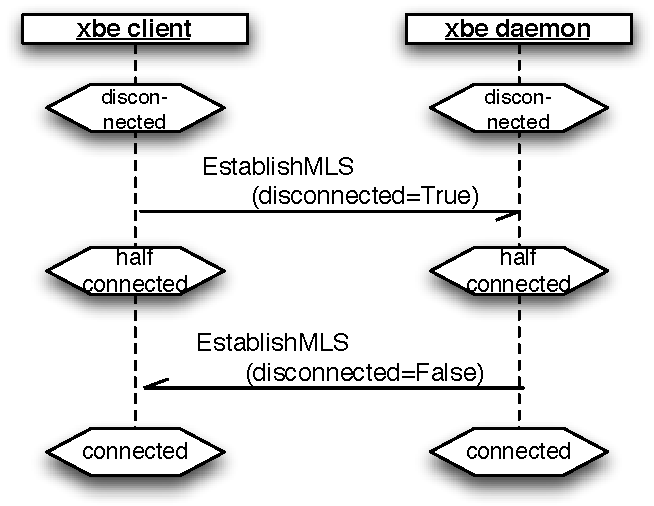
\includegraphics[scale=.75]{msc-establish-mls}
  \end{center}
  \caption[MSC Message Layer Security]{TODO: fill me in}
  \label{fig:msc-establish-mls}
\end{figure}

\begin{figure}
  \begin{center}
    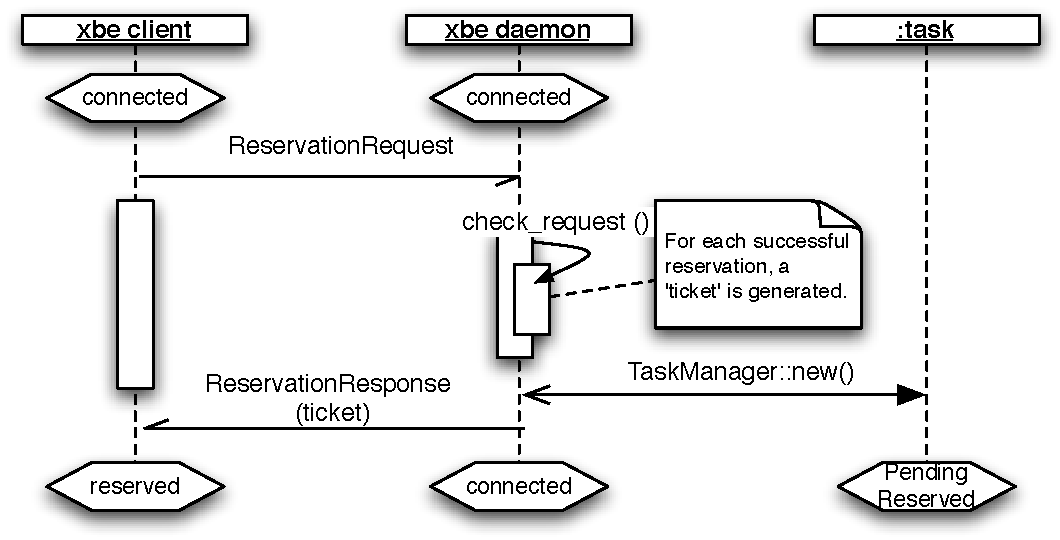
\includegraphics[scale=.75]{msc-reserve}
  \end{center}
  \caption[MSC Make Reservation]{TODO: fill me in}
  \label{fig:msc-reserve}
\end{figure}

\begin{figure}
  \begin{center}
    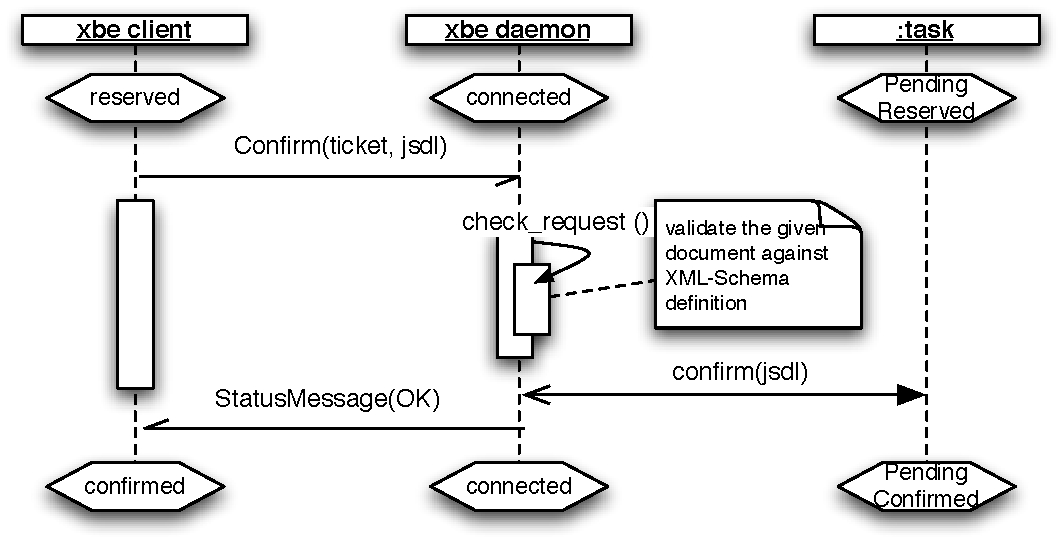
\includegraphics[scale=.75]{msc-confirm}
  \end{center}
  \caption[MSC Confirm Reservation]{TODO: fill me in}
  \label{fig:msc-confirm}
\end{figure}

\begin{figure}
  \begin{center}
    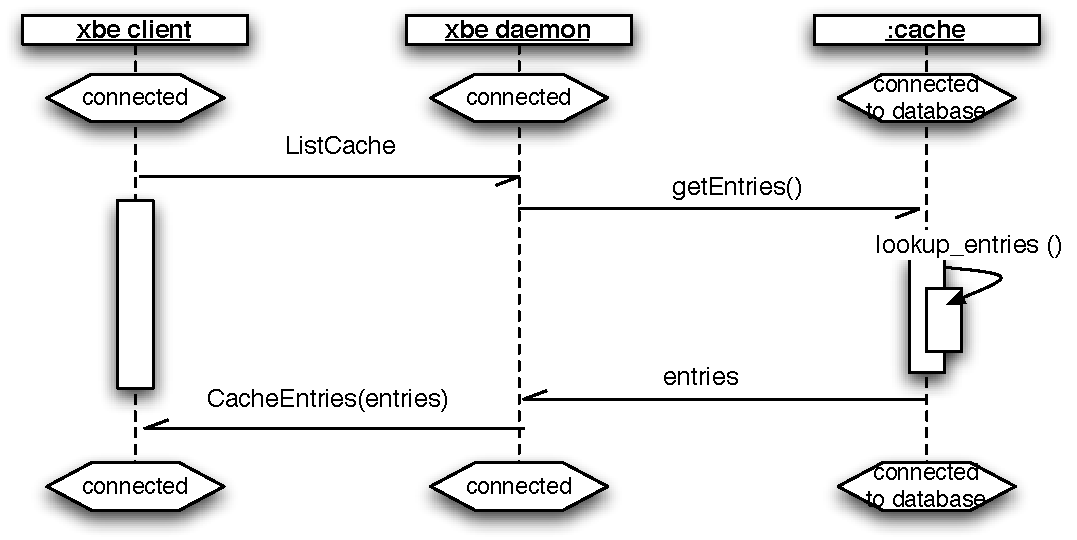
\includegraphics[scale=.75]{msc-list-cache}
  \end{center}
  \caption[MSC List Cache Entries]{TODO: fill me in}
  \label{fig:msc-list-cache}
\end{figure}

\begin{figure}
  \begin{center}
    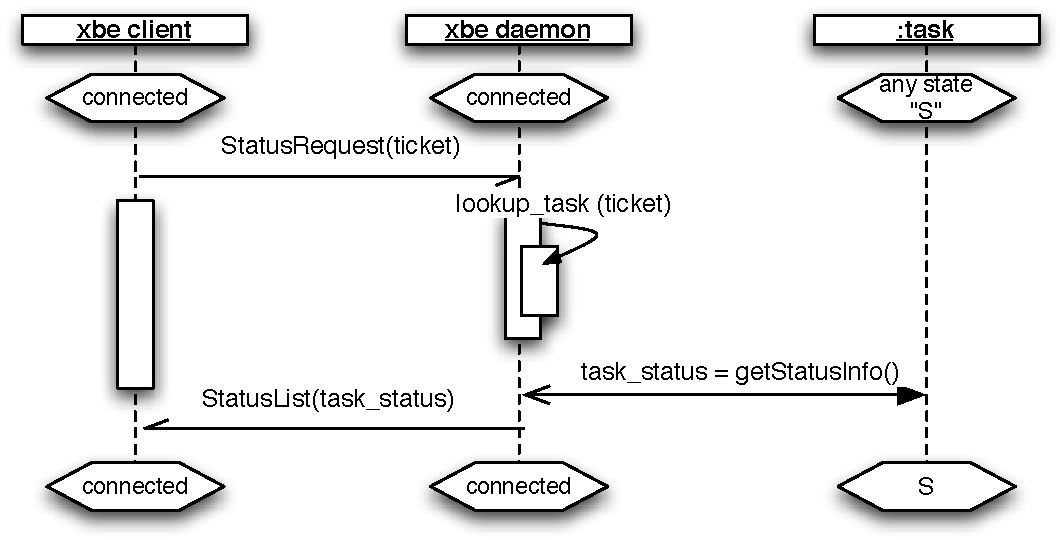
\includegraphics[scale=.75]{msc-status-request}
  \end{center}
  \caption[MSC Request Task Status]{TODO: fill me in}
  \label{fig:msc-status-request}
\end{figure}

\begin{figure}
  \begin{center}
    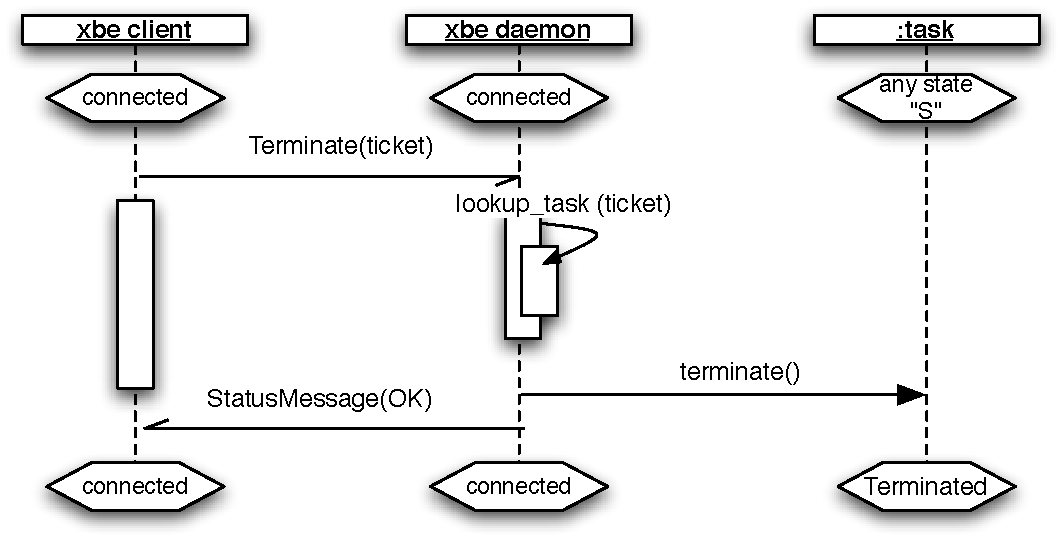
\includegraphics[scale=.75]{msc-terminate}
  \end{center}
  \caption[MSC Terminate Task Request]{TODO: fill me in}
  \label{fig:msc-terminate}
\end{figure}

\begin{figure}
  \begin{center}
    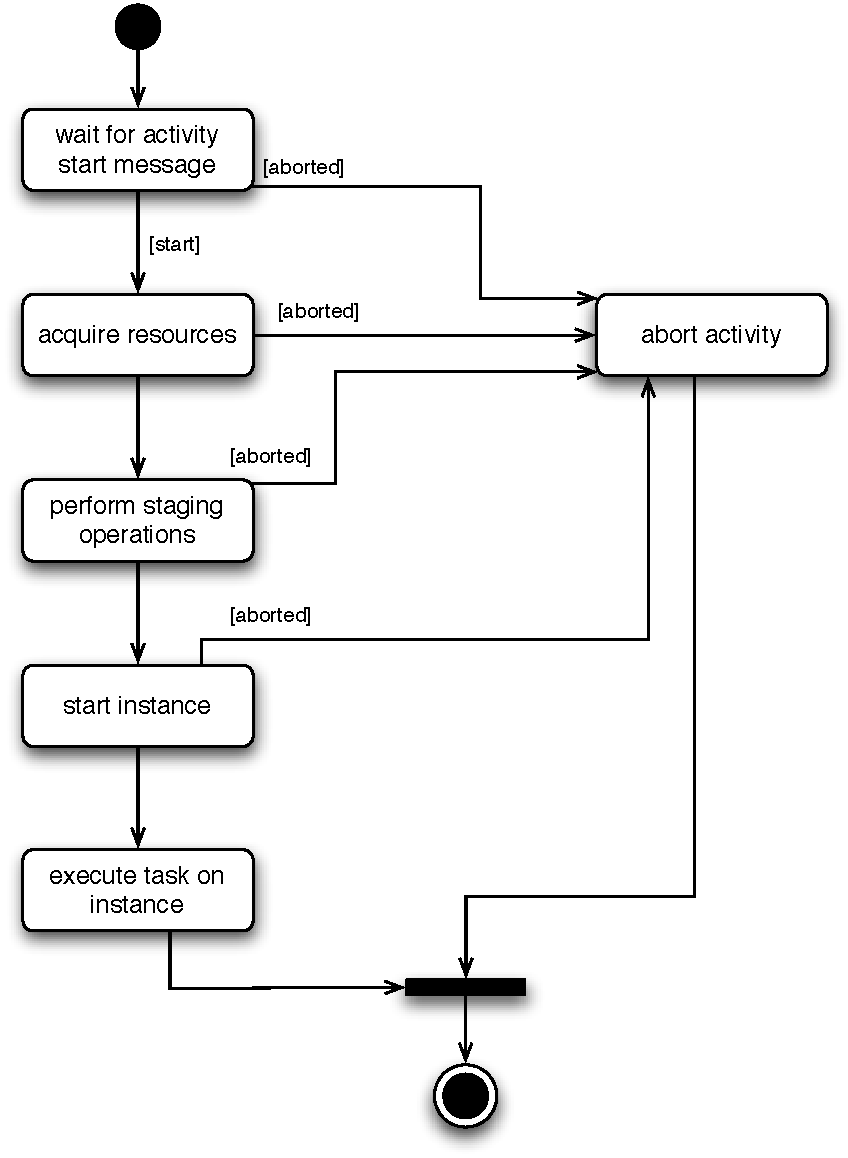
\includegraphics[scale=.75]{act-start-task}
  \end{center}
  \caption[Start Task Activity]{TODO: fill me in}
  \label{fig:act-start-task}
\end{figure}

\begin{figure}
  \begin{center}
    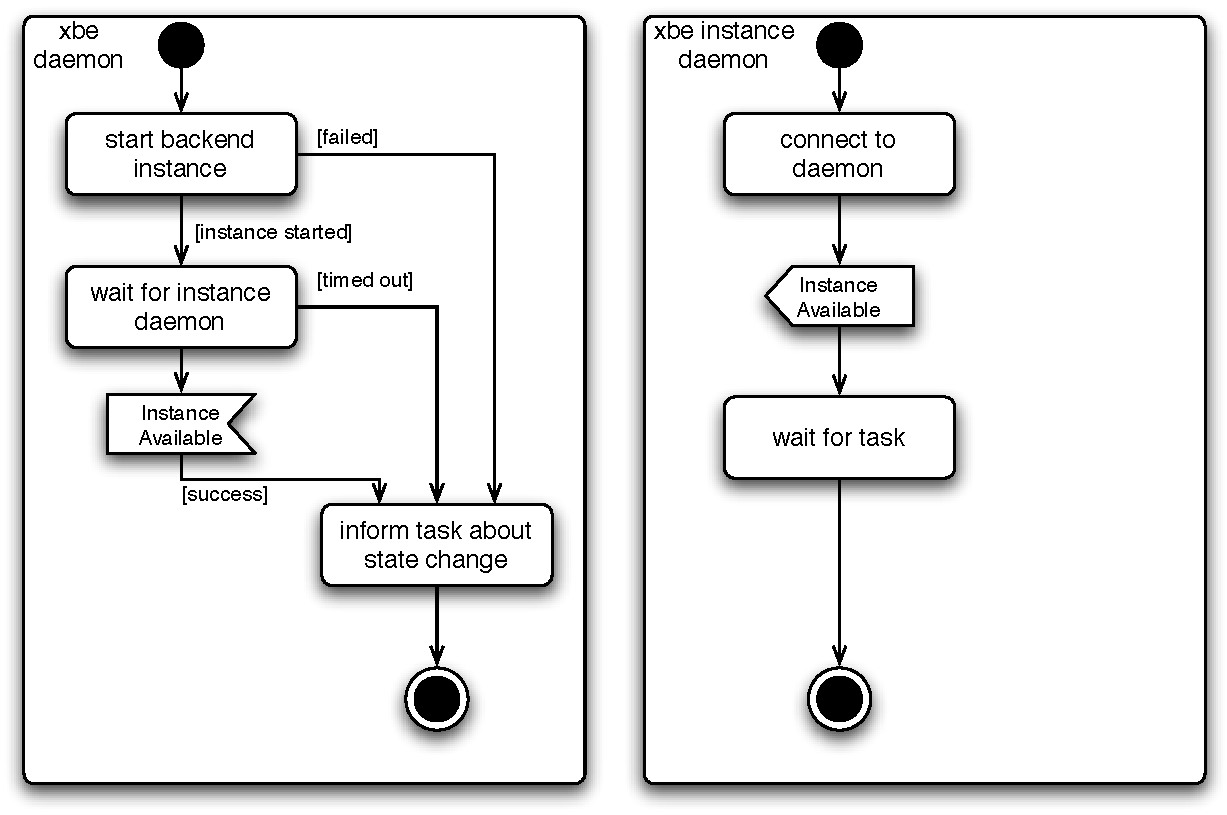
\includegraphics[scale=.75]{act-start-instance}
  \end{center}
  \caption[Start Instance Activity]{TODO: fill me in}
  \label{fig:act-start-instance}
\end{figure}

\begin{figure}
  \begin{center}
    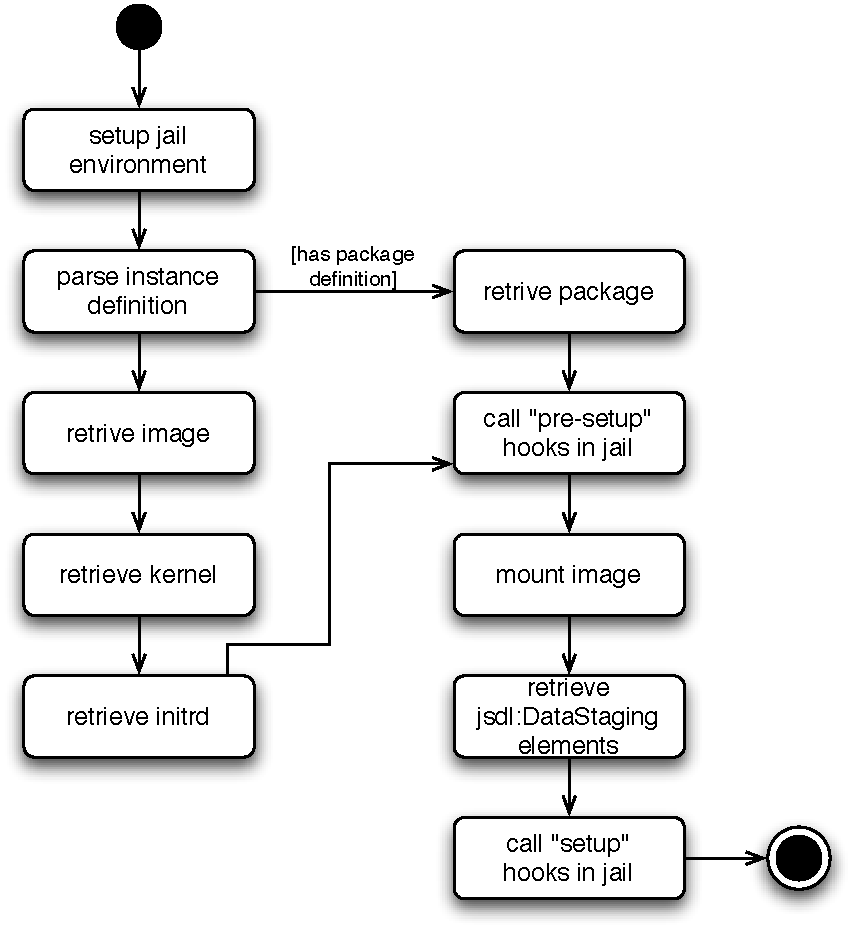
\includegraphics[scale=.75]{act-stage-in}
  \end{center}
  \caption[Stage-In Activity]{TODO: fill me in}
  \label{fig:act-stage-in}
\end{figure}

\begin{figure}
  \begin{center}
    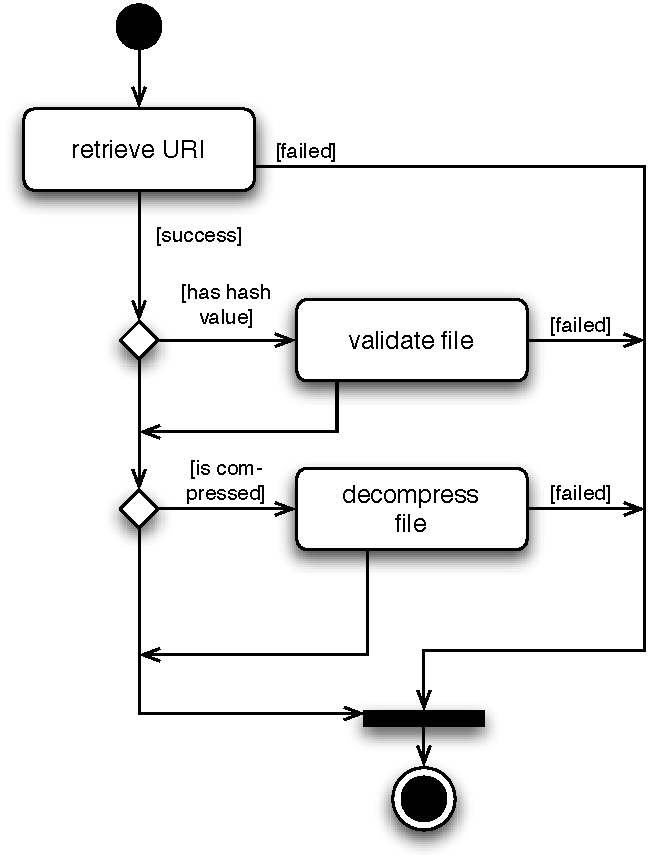
\includegraphics[scale=.75]{act-retrieve-file}
  \end{center}
  \caption[File Retrieval Activity]{TODO: fill me in}
  \label{fig:act-retrieve-file}
\end{figure}


\section{Communication Protocol}
\label{cha:comm-prot}

\subsection{Network Topology}
\label{sec:network-topology}

\begin{figure}
  \begin{center}
    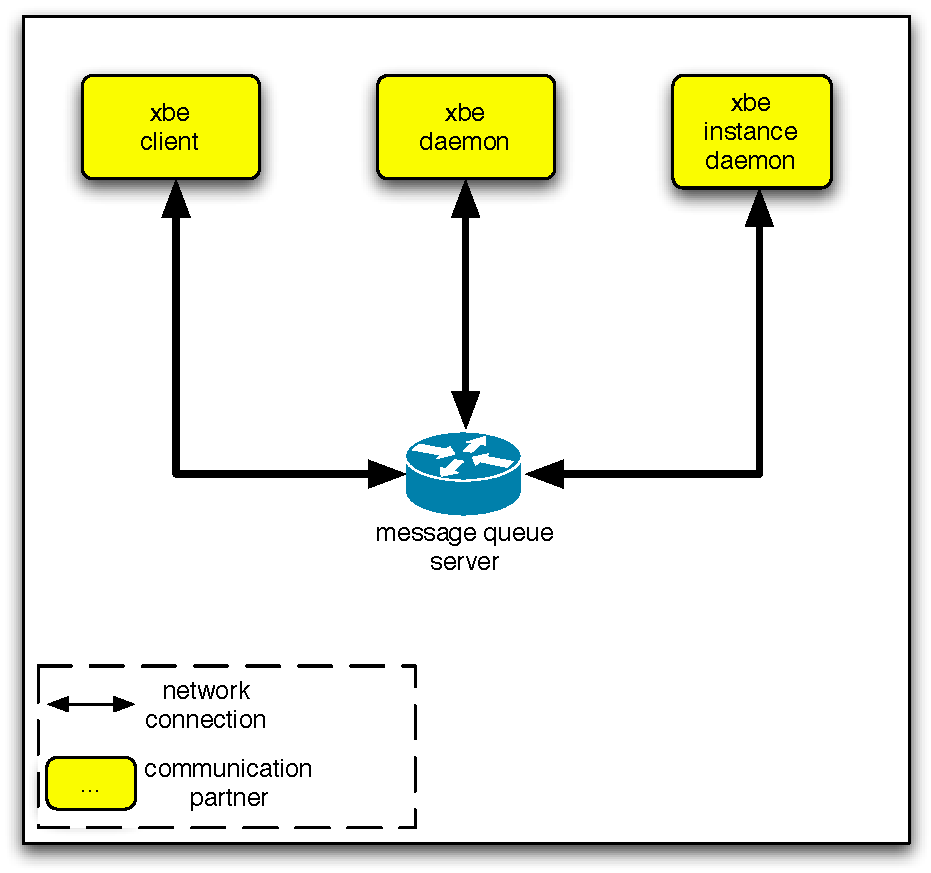
\includegraphics[scale=.75]{simple-network-topology}
  \end{center}
  \caption[Network  Topology   (simple)]{The  simplest  network  topology,
    consisting of  only one Message  Queue Server and  three communication
    partners.}
  \label{fig:simple-net-top}
\end{figure}

\begin{figure}
  \begin{center}
    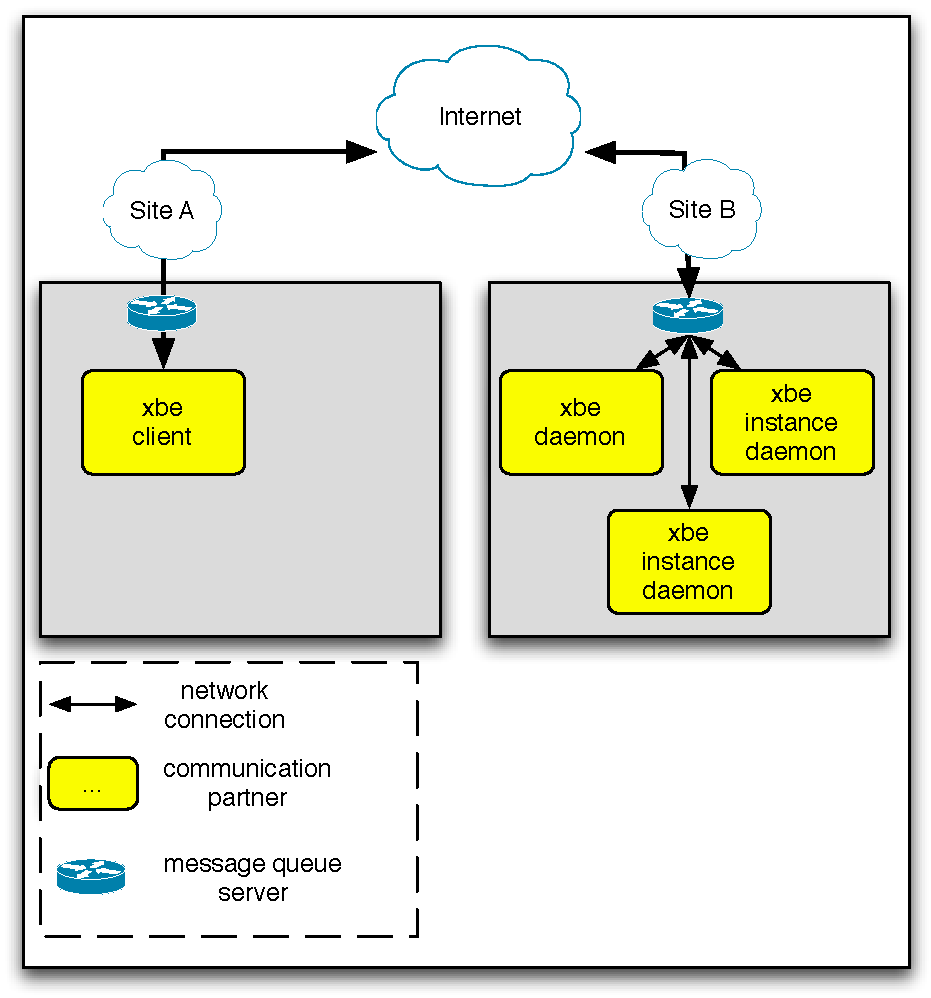
\includegraphics[scale=.75]{network-topology}
  \end{center}
  \caption[Network  Topology]{TODO: fill me in}
  \label{fig:net-top}
\end{figure}

\begin{figure}
  \begin{center}
    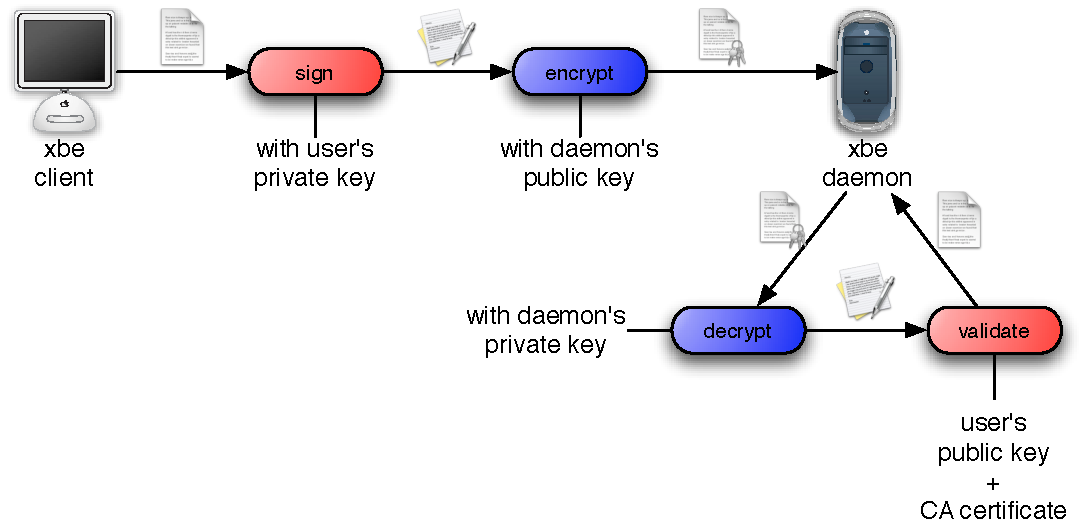
\includegraphics[scale=.75]{message-layer-security}
  \end{center}
  \caption[Message Layer Security]{TODO: fill me in}
  \label{fig:net-mls}
\end{figure}

\begin{figure}
  \begin{center}
    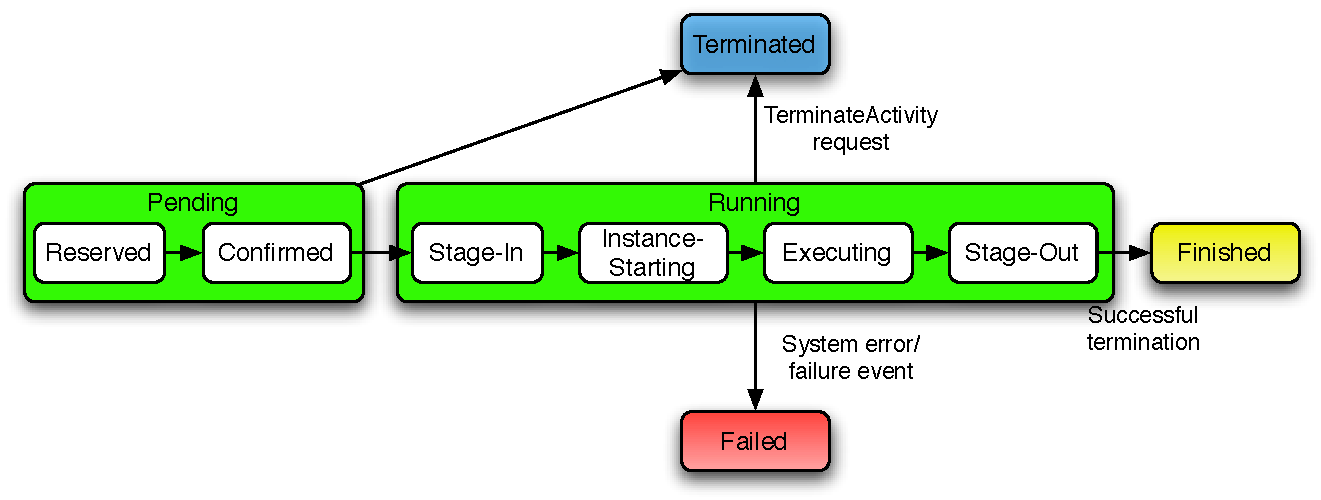
\includegraphics[scale=.75]{extended-job-model}
  \end{center}
  \caption[Job Model (extended)]{TODO: fill me in}
  \label{fig:bes-extended-xen}
\end{figure}

%%% Local Variables: 
%%% mode: latex
%%% TeX-master: "main"
%%% End: 
